In this section we will explain our methodology in more detail. At first we depict our subject, including the open-source projects we choose and the experimental environment we set up. Then we present each step of our approach.

\subsection{Subject systems}

We choose two open-source projects, \emph{Hadoop} and \emph{RxJava} as the subject systems of our case study. \emph{Hadoop}~\cite{hadoop2012:White} is a distributed system infrastructure developed by the Apache Foundation. \emph{Hadoop} performs data processing in a reliable, efficient, high fault tolerance, low cost and scalable manner. We choose \emph{Hadoop} since it is highly concerned with its performance and has been studied in prior research in mining performance data~\cite{markASE}. \emph{RxJava} is a library for composing asynchronous and event-based programs by using observable sequences and it carries the JMH benchmarks test options. \emph{RxJava} is a \emph{Java} VM implementation of reactive extensions. \emph{RxJava} provides a slew of performance micro-benchmarks, making it an appropriate subject for our study. We choose the most recent releases of the two subject systems. The overview of the two subject systems is shown in Table~\ref{tab:subject}. 
\begin{table}[tbh]
	\centering
	\small
	\caption{Overview of our subject systems.}
	\vspace{-0.2cm}
	\label{tab:subject}
	\begin{tabular}{|c|r|r|r|r|}
		\hline
		Subjects                 & Version & \begin{tabular}[c]{@{}c@{}}Total lines\\  of code (K)\end{tabular} & \# files & \# tests \\ \hline
		\multirow{10}{*}{Hadoop} & 2.6.0   & 1,496                                                          & 6,086        & 1,664        \\ \cline{2-5} 
		& 2.6.1   & 1,504                                                          & 6,117        & 1,679        \\ \cline{2-5} 
		& 2.6.2   & 1,505                                                          & 6,117        & 1,679        \\ \cline{2-5} 
		& 2.6.3   & 1,506                                                          & 6,120        & 1,681        \\ \cline{2-5} 
		& 2.6.4   & 1,508                                                          & 6,124        & 1,683        \\ \cline{2-5} 
		& 2.6.5   & 1,510                                                          & 6,127        & 1,685        \\ \cline{2-5} 
		& 2.7.0   & 1,552                                                          & 6,413        & 1,771        \\ \cline{2-5} 
		& 2.7.1   & 1,556                                                          & 6,423        & 1,775        \\ \cline{2-5} 
		& 2.7.2   & 1,562                                                          & 6,434        & 1,784        \\ \cline{2-5} 
		& 2.7.3   & 1,568                                                          & 6,439        & 1,786        \\ \hline
		\multirow{5}{*}{RxJava}  & 2.0.0   & 164                                                            & 1,107        & 76          \\ \cline{2-5} 
		& 2.0.1   & 242                                                            & 1,513        & 76          \\ \cline{2-5} 
		& 2.0.2   & 243                                                            & 1,524        & 76          \\ \cline{2-5} 
		& 2.0.3   & 244                                                            & 1,524        & 76          \\ \cline{2-5} 
		& 2.0.4   & 244                                                            & 1,526        & 76          \\ \hline
	\end{tabular}
	\vspace{-0.4cm}
\end{table}
\subsection{Predicting performance regression introducing changes}
In this subsection, we present our approach of predicting performance regression introducing changes. The overview of our approach is shown in figure~\ref{fig:workflow}.
\begin{figure*}
	\centering
	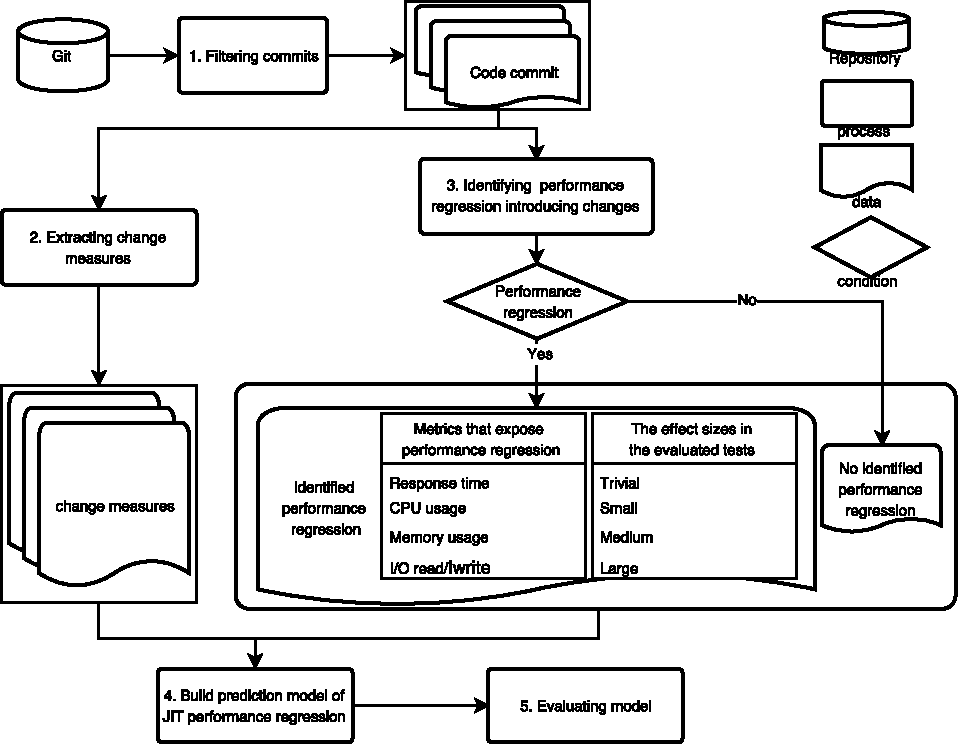
\includegraphics[width=0.85\textwidth]{workflow.pdf}
	\centering \caption{An overview of our approach that predicts performance regression introducing changes}
	\label{fig:workflow}
\end{figure*}
In general, we extract every commit and measures from the version control repositories (Git) of our subject systems and identify impacted test cases of each commit. Afterward, we evaluate performance of each commit using either the related test cases or performance micro-benchmark. Then we perform statistical analysis on the performance evaluation results to identify performance regression. Finally, we build a prediction model based on the change measures to predict the JIT performance regression introducing changes.

\subsubsection{Filtering commits}
As the first step of our approach, we start off by filtering commits in order to focus on commits that are more likely to introduce performance regressions. In particular, we use \emph{git log} command to list all the files that are changed in each commit. We only extract the commits that have source code changes, i.e., changes to \emph{$.$java} files. 

In practice, there may exist multiple commits that are made to accomplish one task, making some of the commits temporary. We would like to avoid considering the performance regressions that are introduced in such temporary commits. Since \emph{Hadoop} uses JIRA as their issue tracking system and \emph{RxJava} uses the internal issue tracking system in Github, we use the issue id that is mentioned in each commit message to identify the task of each commit. If multiple commits are associated with the same issue, we only consider the snapshot of the source code after the last commit. 
\subsubsection{Extracting change measures}
To conduct our research, we extract the domain commit-level change measures and the file-level performance-relevant change measures from the CVS repositories of the projects. The overview of the change measures is shown in Table~\ref{tab:measures}.

 \textbf{Commit-level change measures.} We consider 12 change measures grouped into five dimensions.
\begin{enumerate}[(i)]
	\item \noindent
	\textbf{Diffusion.} We use the diffusion of changes as metrics to indicate the probability that a change can introduce performance regression. In this dimension, first we investigate NS (Number of modified subsystems), ND (Number of modified directories) and NF (Number of modified files). We use \textit{git diff} command to get a list of changed files between every two consecutive commits, including added or deleted lines,  names and pathes of modified files, etc. Then we divide each file path into three parts: subsystem, directory and file, as Fig~\ref{fig:diffusion} shows, name of each subsystem is defined by the root directory name of each path, \textit{.java} file part represents the name of file, and the remaining part in the middle is used to identify the name of a directory. The correspoding measures can be conducted according to their occurance. As for Entropy, we calculate Shannon entropy using the following equations:
	\begin{equation}
		Entropy = - \sum_{i=1}^{n}\left (p_{i}\ast \log_2 p_{i} \right )
	\end{equation}
	\begin{equation}
		p_{i} =\frac{LOC\ changes\ in\ file\ i}{LOC\ changes\ in\ all\ files}
	\end{equation}
	\textit{i} means the number of files, and logarithm is used to normalize the data. Larger entropy value implies more information transmitted, which indicates more changes are caused in this context.
	
	\item \noindent
	\textbf{Size.}
	We use LOC (Lines of Code without comment line and empty lines) as metrics to evaluate the Size changes. LA (LOC added) and LD (LOC deleted) can be obtained directly from the result of \textit{git diff}, and we use \textit{cloc} to get LT (LOC before the change). \textit{cloc} is an open-source project designed to count lines of source code in many programming languages. The larger size of a change,  the higher probability of introducing performance regression.
	
	\item \noindent
	\textbf{Purpose.}
	In this dimension we mainly investigate the rationale of current changes. When programmers decide to change the code, their initial purpose can vary a lot, such as fixing bug, adding new features, improving features, etc.
	However, bug fix sometimes can be a dangerous action because it may unintentionally introduce new defects, which have high probability to cause performance regression. In our approach, we use issue tracking systems to define whether the type of current commit is a bug fixing. We use \textit{JIRA}, a widely adopted commercial issue tracking system, to gather information about hadoop commits. Unlike hadoop, Rxjava does not have its own independent JIRA database, but we can also fetch detailed issue reports from Github for further analysis. We use scripts to crawl issue type of each commit from both JIRA and Github, because their information is authentic and up to date. Then we can determine whether a change is because of bug fixing or not.
	
	\item \noindent
	\textbf{History.}
	In History dimension, we mainly discuss two kinds of change measures: NDEV (The number of developers touched a file) and AGE (The average time interval between last and current change). Previous findings indicate that files touched by more people are more likely to introduce a problem\cite{matsumoto2010analysis}, and recent changes are easier to cause faults\cite{eick2001does}. Those unexpected deficiencies, as by-product brought by changes, are highly risky to cause performance degradations. We use \textit{git blame} command followed by touched file name, this will display who and when was each line of code touched. We count the number of different developers to obtain NDEV value. As for AGE, because we already have a list of touched files between two consecutive commits, we calculate the average time of each file and save them into a list. Because the value of time parameter is relatively large, so we need to preprocess our data before we continue our analysis.We use the following formula to normalize and rescale the data.
	\begin{equation}
		AGE = \frac{T_{Avg}-T_{Min}}{T_{Max}-T_{Min}}
	\end{equation}
	The three parameters in the equation refer to the average, maximum and minimum number in previous list. 
	
	\item \noindent
	\textbf{Experience.}
	The Experience dimension is to evaluate the programmer familiarity with the system. In our study, we mainly consider EXP (Developer experience) and REXP (Recent developer experience) as important indicators to quantify programmers' experience with a system. Increasing familiarity can reduce the likelihood of making mistakes\cite{mockus2000predicting}, and experienced specialists can capture "best practice" in software design to diminish software performance problems\cite{smith2003more}. Because all of our commits are from most recent releases, we acquire information of all contributors from  \textit{Open Hub}, a public directory of open source software with up to date information. Those information contains the total number of commits to a project, and the number of commits within recent 12 months, which can act as measures to developers' experience in our study. We crawl EXP and REXP data of all the contributors from \textit{OpenHub} and save them into different local files, the next step is to match contributor information to different commits. For RxJava, first we use \textit{git log} command to acquire all the commits and name of contributors. Therefore, we can merge those results into a larger local dataset according to name matching, and we can query information of contributors from it using commits. However, the situation in hadoop is completely different. Unlike Rxjava, there exists an agency between contributors and source repository. The middle layer is called Hadoop Project Management Committe (PMC), which contains people with direct access to hadoop repository. When programmers want to make a change in hadoop, their changes will be reviewed by a PMC member to ensure the quality. If it is approved, the committer will submit to hadoop repository with information \textit{"Contributed by RealContributorName"}. In consequent, from git command we can hardly tell the real contributor of a commit because only the information of commiter will be shown. So we crawling names of real contributors from JIRA and query contributor experience data from local file by name matching. 
	
	
	\begin{figure}
		\centering
		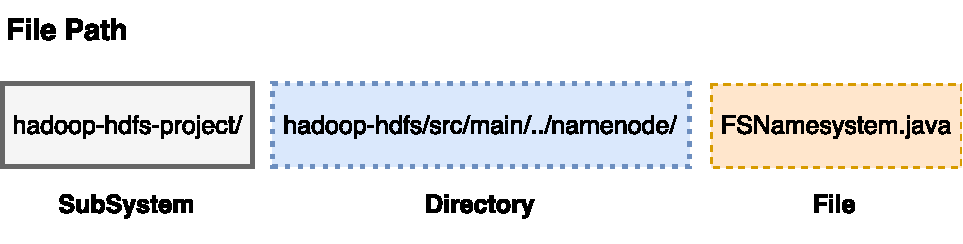
\includegraphics[width=\columnwidth]{Diffusion.pdf}
		\centering \caption{The division of file path}
		\label{fig:diffusion}
	\end{figure}
\end{enumerate}

\textbf{Performance-relevant change measures.} Simultaneously, we extract performance-relevent change measures automatically, including CC (changing conditions), CL (changing loops), FC (changing function calls), IL (Introducing locks and synchronization) and EV (expensive variables). The first three measures are most relevent to performance~\cite{ACM2016:Luo}. Also, after we find the performance regression we check the source code manully and find that IL and EV are also the most root-cause of regression. 

CC can change the code that is executed and may cause more operation eventually executed by the software, leading to performance regressions. CL may significantly slow down performance. Locks are expensive actions for software performance. IL means that introducing locks and synchronization can suspend threads waiting on a lock until released, causing performance degradation on response time.  For example, in commit \#2946621a in Hadoop, developers added synchronized operation to lock the block in class Met- ricsSourceAdapter.java, in order to protest the shared resources used by the two functions inside the block (see figure~\ref{fig:1b}). FC is that developers may introduce expensive function calls with the function execution expensive by itself or executed a large number of time. For example, in class Mover.java of commit \#c927f938 in Hadoop. Developers added an API call shuffle of Collections inside a loop, leading to the performance regression (see figure~\ref{fig:1a}).
EV means that some variables are more expensive to be held in memory and need more resources to visit or operate. 

\begin{figure*}
	\centering
	\begin{subfigure}{\textwidth}% -----------------------------------------1111111one code pair
		\begin{subfigure}{0.51\textwidth}
			\begin{lstlisting}[language=Java]
			for (StorageType t : targetTypes) {																		
			-  for(StorageGroup target:storages.getTargetStorages(t)) {
			
			
			if (matcher.match(cluster, source.getDatanodeInfo(),
			target.getDatanodeInfo())) {
			final PendingMove pm = source.addPendingMove(db, target);
			\end{lstlisting}
		\end{subfigure}
		\begin{subfigure}{0.51\textwidth}
			\begin{lstlisting}[language=Java]
			for (StorageType t : targetTypes) {																		
			+ final List<StorageGroup> targets=storages.getTargetStorages(t);
			+ Collections.shuffle(targets); 
			+ for (StorageGroup target : targets) {
			if (matcher.match(cluster, source.getDatanodeInfo(),
			target.getDatanodeInfo())) {
			final PendingMove pm = source.addPendingMove(db, target);
			\end{lstlisting}
		\end{subfigure}
		\caption{Code change of changing function call in issue \#HDFS-10335 of commit \#c927f938}\label{fig:1a}
	\end{subfigure}
	\vspace*{\fill} % separation between the subfigures
	\begin{subfigure}{\textwidth}% ----------------------------------------555555555 one code pair
		\begin{subfigure}{0.51\textwidth}
			\begin{lstlisting}[language=java]
			
			updateAttrCache();
			if (getAllMetrics) {		       
			updateInfoCache();		       
			}
			\end{lstlisting}
		\end{subfigure}
		\begin{subfigure}{0.51\textwidth}
			\begin{lstlisting}[language=Java]
			+  synchronized(this) {
			updateAttrCache();
			if (getAllMetrics) {		       
			updateInfoCache();		       
			}
			\end{lstlisting}
		\end{subfigure}
		\caption{Code change of introducing synchronization in issue \#HADOOP-11361 of commit \#2946621a}\label{fig:1b}
	\end{subfigure}
	\caption{Examples of performance regression introducing changes} \label{fig:example}
\end{figure*}

To extract performance-relevant change measures, we only need to focus on the file corresponding test case. We utilize tool \emph{srcML}~\cite{srcml_2017} to convert the source code of the same file from current commit and its parent commit to XML file. Afterward, we employ \emph{diff} tool and regular expression to compare the source code.

\begin{table}[]
	\centering
	\small
	\caption{Summary of domain and performance-relevant change measures}
	\label{tab:measures}
\begin{tabular}{|l|l|l|}
	\hline
	Dim.                         & Name    & Definition                                                                                                   \\ \hline
	\multirow{4}{*}{Diffusion}   & NS      & Number of modified subsystems                                                                                \\ \cline{2-3} 
	& ND      & Number of modified directories                                                                               \\ \cline{2-3} 
	& NF      & Number of modified files                                                                                     \\ \cline{2-3} 
	& Entropy & Distribution of modified code across files                                                                   \\ \hline
	\multirow{3}{*}{Size}        & LA      & Lines of code added                                                                                          \\ \cline{2-3} 
	& LD      & Lines of code deleted                                                                                        \\ \cline{2-3} 
	& LT      & Lines of code before the change                                                                              \\ \hline
	Purpose                      & FIX     & Whether or not the changes fix a bug                                                                    \\ \hline
	\multirow{2}{*}{History}     & NDEV    & \begin{tabular}[c]{@{}l@{}}Number of developers that changed \\ the modified files\end{tabular}              \\ \cline{2-3} 
	& AGE     & \begin{tabular}[c]{@{}l@{}}The average time interval between the \\ last and the current change\end{tabular} \\ \hline
	\multirow{2}{*}{Experience}  & EXP     & Developer experience                                                                                         \\ \cline{2-3} 
	& REXP    & Recent developer experience                                                                                  \\ \hline
	\multirow{5}{*}{Perf.} & CC      & Number of changing condition                                                                                 \\ \cline{2-3} 
	& CL      & Number of changing loop                                                                                      \\ \cline{2-3} 
	& IL      & \begin{tabular}[c]{@{}l@{}}Number of introducing locks or \\ synchronization\end{tabular}                    \\ \cline{2-3} 
	& EV      & Number of expensive variable                                                                         \\ \cline{2-3}
	& FC      & Number of changing function call                                                                             \\ \hline
\end{tabular}
\end{table}
\subsubsection{Identification of  performance regression introducing changes}
In more detail, we give a list of particular step:
%\begin{enumerate}[(i)]
%\item 

\textbf{Identifying impacted tests.} In order to evaluate performance of each code commit, we use the tests and performance micro-benchmarks that are readily available in the source code of our subject systems. As mature software projects, each subject system consist of a large amount of test cases. 
For example, \emph{Hadoop} release2.7.3 contains 1786 test cases in total. Exercising all test cases may cause two issues to our performance evaluation: 1) the test cases that are not impacted by the code change would dilute the performance impact from the code changes and introduce noise in the performance evaluation and 2) the large amounts of un-impacted test cases would requires extra resources for performance evaluation (e.g., much longer test running time). 

Therefore, in this step, we leverage a heuristic to identify impacted tests for each commit. In particular, we find that \emph{Hadoop} test cases follow a naming convention that the name of the test files contain that same name of the source code files being tested. For example, a test file named \emph{TestFSNamesystem.java} tests the functionality of \emph{FSNamesystem.java}. Hence, for each changed source code file in a commit, we automatically identify the test files. 

\textbf{Dealing with changed tests.} Some commits may change source code and test code at the same time. Such changed test cases would bias the performance evaluation if much testing logic is added, removed or modified in the test cases. In order to minimize the impact of changed test cases in performance evaluation, we opt to use the test code before the code change, since the new version of the test cases may include new features of the system, which is not the major concern of performance regression. However, in the cases where old test cases cannot compile or failed, we use the new test cases, since the failure of the compilation or the tests indicates that the old feature may be outdated. Finally, if both new and old test cases are failed or un-compliable, we do not include this test in the performance evaluation. In total, we have 132 tests with 106 commits that use the new tests to evaluate performance and 21 test with 19 commits that are not included in our performance evaluation. There exist only six commits that are not included at all because all of their tests are either un-compliable or failed.

\textbf{Leveraging micro-benchmarks for \emph{RxJava}. }Fortunately, \emph{RxJava} provides a slew of micro-benchmarks with the goal of easing performance evaluation. We find that these performance micro-benchmarks are designed to evaluate performance of the software as a cross-cutting concern, instead of evaluating any particular features separately. Therefore, we opt to run all 76 micro-benchmarks from \emph{RxJava}. In the rest of this paper, we also refer these micro-benchmarks as test cases to ease the description of our results.

%\item 
\textbf{Evaluating performance.}
In this step, we exercise the prepared test cases and the performance micro-benchmarks to evaluate performance of each commit. We setup our performance evaluation environment based on Azure node type Standard F8s (8 cores, 16 GB memory). In order to generate statistically rigorous performance results, we adopt the practice of repetitive measurements~\cite{peterfse} to evaluate performance. 
In particular, each test or performance micro-benchmark are executed 30 times independently. We collect both domain level and physical level performance metrics during the tests. We measure the response time of each test case as domain level performance metric. A shorter response time indicating better performance of the software. We use a performance monitoring software named \emph{psutil}~\cite{psutil} to monitor physical level performance metrics, i.e., the CPU usage, Memory usage, I/O read and I/O write of the software, during the test.

%\item 
\textbf{Statistical analyses on performance evaluation.}
Statistical tests have been used in prior research and in practice to detect whether performance metric values from two tests reveal performance regressions \cite{AlGhmadi}. After having the performance evolution results, we perform statistical analyses to determine the existence and the magnitude of performance regression in a statistically rigorous manner. 
We use Student’s t-test to examine if there exists statistically significant difference (i.e., p-value $<$ 0.05) between the means of the performance metrics. A p-value $<$ 0.05 means that the difference is likely not by chance. 
A t-test assumes that the population distribution is normally distributed. Our performance measures should be approximately normally distributed given the sample size is large enough according to the central limit theorem \cite{Chen:2014}.
T-test would only tells us if the differences of the mean between the performance metrics from two commits are statistically significant. On the other hand, effect sizes quantify such differences. 

Researchers have shown that reporting only the statistical significance may lead to erroneous results (i.e., if the sample size is very large, p-value can be small even if the difference is trivial). We use \emph{Cohen\textquotesingle s d} to quantify the effects~\cite{ES2006:Becker}. \emph{Cohen\textquotesingle s d} measures the effect size statistically and has been used in prior engineering studies~\cite{IST2007:Kampenes, ICSE2002:Kitchenham}. \emph{Cohen\textquotesingle s d} is defined as:
$$
Cohen\textquotesingle s \ d=\frac{mean(x1)-mean(x2)}{s}
$$
where \emph{mean(x1)} and \emph{mean(x2)} are the mean of two populations, and s is the pooled standard deviation~\cite{JohnWiley:2011}.
$$
\mathit{effect \ size} = \left\{ \begin{array}{ll}
trivial & \textrm{if $Cohen\textquotesingle s \ d  \leqslant 0.2$}\\
small & \textrm{if $0.2 < Cohen\textquotesingle s \ d \leqslant 0.5$}\\
medium& \textrm{if $0.5 < Cohen\textquotesingle s \ d \leqslant 0.8$}\\
large& \textrm{if $0.8 < Cohen\textquotesingle s \ d$}
\end{array} \right.
$$

%\end{enumerate}
\subsubsection{Data Preprocessing}
Before utilize the attributes to build our prediction models, we need to employ data preprocessing to make sure the data quality, including accuracy, completeness, consistency and timeliness. In our project, we perform data cleaning to fill in missing values, data transformation to normalize the raw data, and remove redundant data.

Missing value happens in the \emph{FIX, EXP and REXP} in our study. Because a few commits without issue report so we cannot extract the purpose of this commit (FIX). And a few commits' contributors are not in the \emph{Hadoop} contributor official list~\cite{hadoop_2017} so we cannot calculate the measures EXP and REXP. In this case, we use a global constant to fill in the missing value. We replace all missing values by the same constant ``Unknown`` and ``1`` in measure FIX and EXP \& REXP, respectively.

Data normalization or standardization can help avoid data skew and give all measures an equal weight. The values of different attributes may have large different range due to various measurement units. It tends to give such an attribute with smaller units greater effect or weight. In particular, we perform \emph{Min-max normalization} to transform our original data.

Redundancy is an essential issue in the data integration, which means that a measure may be redundant if it is derived from another measure or a set of measures. We employ correlation analysis to remove highly correlated measures. In particular, we use \emph{Correlation-based Feature Selection} and \emph{Information Gain Rate} technique to solve this problem.

\subsubsection{Build prediction model of JIT performance regression}

\textbf{Model building.} First, we want to build logistic regression model to predict the existence of performance regression introducing change. We choose logistic regression model because it is easy to interpre. Second, we build a ordinal model to predict the effect size of performance regression. Our ordinal class consists of not significant difference, small, medium and large regression. Standard classification algorithms consider the class value as a nominal quantity so that it cannot operate this ordering information. Thrid, we use the coefficient and odds ratio to compare and find the important change measures of performance regression.


\textbf{Model evaluation.} We utilize three metrics to evaluate classifier performance, including \emph{precision}, \emph{recall} and \emph{AUC}~\cite{Fawcett2006ROC}. It depends on confusion matrix which contains four terms consisting of \emph{true positives, true negatives, false positives and false negatives}. 
We perform stratified k-fold cross-validation for estimating accuracy and determine the \emph{k} as 10 due to its relatively low bias and variance.

In particular, we use the most popular machine learning tool \emph{Weka}~\cite{Hall:2009:weka} to train the dataset and build the corresponding model. Fristly we build the model and predict the text data within project. Afterward, we employ the model to predict text data cross-project.

